\documentclass[]{report}

\voffset=-1.5cm
\oddsidemargin=0.0cm
\textwidth = 480pt

\usepackage{framed}
\usepackage{subfiles}
\usepackage{graphics}
\usepackage{newlfont}
\usepackage{eurosym}
\usepackage{amsmath,amsthm,amsfonts}
\usepackage{amsmath}
\usepackage{color}
\usepackage{amssymb}
\usepackage{multicol}
\usepackage[dvipsnames]{xcolor}
\usepackage{graphicx}
\begin{document}
%-----------------------------------------------------------------%

\chapter{Regression}



			\section{Introduction to Regression}
			
			\begin{itemize}
				\item Linear regression is used when you want to predict the value of a variable based on the value of another variable. The variable we want to predict is called the dependent variable (or sometimes, the outcome variable). The variable we are using to predict the other variable's value is called the independent variable (or sometimes, the predictor variable).
				
				
				\item For example, you could use linear regression to understand whether exam performance can be predicted based on revision time; whether cigarette consumptions can be predicted based on smoking duration; and so forth. If you have two or more independent variables, rather than just one, you need to use \textbf{\textit{multiple regression}}.
				
				\item	\texttt{R} can be used to carry out linear regression, as well as interpret and report the results from this test. However, before we introduce you to this procedure, you need to understand the different assumptions that your data must meet in order for linear regression to give you a valid result. We discuss these assumptions next.
				
			\end{itemize}
			
			
			
			









%---------------------------------------------------------------------%

\section{Regression Equation}
A regression equation allows us to express the relationship between two (or more) variables algebraically. It indicates the nature of the relationship between two (or more) variables. In particular, it indicates the extent to which you can predict some variables by knowing others, or the extent to which some are associated with others.



A linear regression equation is usually written
\[Y = a + bX + e\]
where
\begin{itemize}
	\item Y is the dependent variable
	\item a is the intercept
	\item b is the slope or regression coefficient
	\item X is the independent variable (or covariate)
	\item e is the error term
\end{itemize}
The equation will specify the average magnitude of the expected change in Y given a change in X.

The regression equation is often represented on a scatterplot by a regression line.

					\section{Regression}
					
					\begin{itemize}
						\item Consider two populations X and Y that are indepedently distributed from
						each other.
						\item That is to say, the true value of correlation is zero.
						\[\rho_{XY} = 0 \]
						\item In the context of a linear regression model, in the form $Y=\beta_0  +  \beta_1X$, a true correlation value of zero is equivalent to a true slope value of Zero.
						\["\rho_{XY} = 0" \rightarrow\leftarrow "\beta_1=0"\]
					\end{itemize}
					

					%-------------------------------------------%
					

\subsection{Regression}
A statistical measure that attempts to determine the strength of the relationship between one dependent variable 
(usually denoted by Y) and a series of other changing variables (known as independent variables).

Regression takes a group of random variables, thought to be predicting Y, and tries to find a mathematical relationship between them. This relationship is typically in the form of a straight line (linear regression) that best approximates all the individual data points.



%---------------------------------------------------------------------%

\subsection{Regression}

Two events can consistently correlate with each other but not have any causal relationship. 
An example is the relationship between reading ability and shoe size across the whole population of the United States. 
If someone performed such a survey, they would find that the larger shoe sizes correlate with better reading ability, but 
this does not mean large feet cause good reading skills. Instead it's caused by the fact that young children have small 
feet and have not yet (or only recently) been taught to read. In this case, the two variables are more accurately correlated with a third: age.

%---------------------------------------------------------------------%


\subsection{Least Squares}
The method of least squares is a criterion for fitting a specified model to observed data. 
For example, it is the most commonly used method of defining a straight line through a set of points on a scatterplot.



%------------------------------------------------------- %

\subsection{Regression Equation}
A regression equation allows us to express the relationship between two (or more) variables algebraically. It indicates the nature of the relationship between two (or more) variables. In particular, it indicates the extent to which you can predict some variables by knowing others, or the extent to which some are associated with others.



A linear regression equation is usually written
\[Y = a + bX + e\]
where
\begin{itemize}
	\item Y is the dependent variable 
	\item a is the intercept 
	\item b is the slope or regression coefficient 
	\item X is the independent variable (or covariate) 
	\item e is the error term 
\end{itemize}
The equation will specify the average magnitude of the expected change in Y given a change in X.

The regression equation is often represented on a scatterplot by a regression line.



	\section{Simple Linear Regression }
	\begin{itemize}
		\item 
		Simple linear regression is used for testing hypotheses about the relationship between a dependent variable $Y$ and an independent prediction variable $X$.
		
		\item 	Simple linear regression is also used to predicted a value of Y for a given X. Predictions are only valid for X values inside 
		the current range of $X$ values. 
		
		\item 	An Error term measures the deviation of each observed value from the true (but unobserved) regression line.
		A residual measures the deviation of each observed value for the fitted line.
		
		\item 	The ordinary least squares (OLS) method gives the best straight line that fits the observations, by minimizing the sum of the
		squared vertical deviations of each deviations of eahc observation from the fitted line.
		\item The coeffcieint of determination $R^2$ is defined as the proportion of variation of Y explained by the regression of Y on X. $R^2$ is dimensionless, and takes a value between 0 and 1.
		
		\item 	Correlation coefficients measure the degree of association between two variables. The coefficient takes a value between -1 and 1.
		
		\item 	an estimator is unbiased if the mean of its sampling distribution is equal to the true parameter.
	\end{itemize}
	
%----------------------------------------------------------- %

\section{Simple Linear Regression}
We consider the simplest type of regression line where there are only two
variables
\begin{itemize}
	\item  one response variable (Y)
	\item one predictor variable (X)
\end{itemize}
This is called Simple Linear Regression and the mathematical model is:
\[ Y = \beta_0 + \beta_1X + \epsilon \]

The true values of $\beta_0$ and  $\beta_1$ are almost always unknown, but are instead estimated from sample data.

%---------------------------------------------------------------------%	
	

\section{Regression Line}




A regression line is a line drawn through the points on a scatterplot to summarise the relationship between the variables being studied. When it slopes down (from top left to bottom right), this indicates a negative or inverse relationship between the variables; when it slopes up (from bottom right to top left), a positive or direct relationship is indicated.

The regression line often represents the regression equation on a scatterplot.



\section*{Objectives \& Assumptions} 

The primary objective of regression analysis is to estimate the value of a random variable (the dependent
variable) given that the value of an associated variable (the independent variable) is known. 

\begin{itemize}
	\item The dependent
	variable is also called the response variable, while the independent variable is also called the predictor
	variable. 
	
	\item The regression equation is the algebraic formula by which the estimated value of the dependent, or
	response, variable is determined.
	\item The term simple regression analysis indicates that the value of a dependent variable is estimated on the
	basis of one independent, or predictor, variable.
	
	\item \textit{\textbf{Multiple regression analysis}} is
	concerned with estimating the value of a dependent variable on the basis of two or more independent variables.
\end{itemize}



\section{Examples}
%-------------------------------------------------%



% X = c(40,28,34,27,21,38,19,45,31,35)
% Y = c(1,6,6,9,12,4,13,2,5,3)





%-------------------------------------------------%

\subsection{Example 2 Part 2}
\begin{itemize}
	\item Calculate the slope estimate for the regression equation.
	\item The slope estimate is computed using the following formula:
	\[ b_1 = \frac{\S_{XY}}{S_{XX}} \]
	\item From the values given
	\[ b_1 = \frac{-283.8}{613.6} =-0.4625 \]
	\item 
\end{itemize}




	\section*{Linear Regression}
	\begin{itemize}
		\item Linear regression is the most widely used of all statistical techniques: it is the study of linear (i.e., straight-line) relationships between variables, usually under an assumption of normally distributed errors.
	\end{itemize}


\section{Simple Linear Regression}
\begin{itemize}
\item	We have to find the line of best fit. Before we can do this, we must assume that one
		variable is dependent on the other. 
		
	\item The theory we learn here assumes we are going to use a straight line, and not a curve of any kind, though in some disciplines (physics or finance, for example) a curve would be more appropriate.
	
	\item We have to find the line of best fit. Before we can do this, we must assume that one
	variable is dependent on the other. By convention we call the dependent variable y
	and the independent variable x. We have to work out the slope of the line, and the
	point at which it cuts the y axis.
	
	\item Again, by convention, we call these values and respectively for the population.
	
	\item The basic model is therefore given as follows.
	
	\item The model of a random variable Y, the dependent variable, which is related to random
	variable X, the independent (or predictor or explanatory) variable by the equation:
	\begin{equation}
	Y = \alpha + \beta X + \epsilon
	\end{equation}
	
	where $\alpha$ and $\beta$ are constants and $\epsilon ~ N ( 0,\sigma^2)$ , a random error term. The
	coefficients $\alpha$ and $\beta$  are theoretical values and can only be estimated from sample data.
\end{itemize}

\begin{itemize}

	\item By convention we call the dependent variable y
	and the independent variable x. We have to work out the slope of the line, and the
	point at which it cuts the y axis.
	
	\item	Again, by convention, we call these values and respectively for the population.
\end{itemize}

The estimates are generally written as $a$ and $b$.

Given a sample of bivariate data, $(x_1,y_1),(x_2,y_2) ,.........., (x_n,y_n)$, $a$ and $b$ can be
estimated. To fit a line to some data as in this case, an objective must be chosen to
define which straight line best describes the data. The most common objective is to
minimise the sum of the squared distance between the observed value of $y_i$
and the corresponding predicted value $\hat{y}_i$.

The estimated least squares regression line is written as:
$y = a + b\times x$
We can derive the formulae for $b$ and $a$.



The line is called the sample regression line of y on x.

The following example demonstrates the calculation of a and b and the use of the resultant
equation to estimate y for a given x.

\newpage


	
\begin{itemize}
\item 	The estimates are generally written as $a$ and $b$.
\item 	Given a sample of bivariate data, $(x_1,y_1),(x_2,y_2) ,.........., (x_n,y_n)$, $a$ and $b$ can be
	estimated. 
\item  To fit a line to some data as in this case, an objective must be chosen to
	define which straight line best describes the data. 
\item  The most common objective is to
	minimise the sum of the squared distance between the observed value of $y_i$
	and the corresponding predicted value $\hat{y}_i$.
\item 	The estimated least squares regression line is written as:
	$y = a + b\times x$
	We can derive the formulae for $b$ and $a$.
\item 	The line is called the sample regression line of y on x.
\item 	The following example demonstrates the calculation of a and b and the use of the resultant
	equation to estimate y for a given x.
\end{itemize}

	
%---------------------------------------------------------------------%


\section{Regression}
We consider the simplest type of regression line where there are only two
variables
\begin{itemize}
	\item  one response variable (Y)
	\item one predictor variable (X)
\end{itemize}
This is called Simple Linear Regression and the mathematical model is:
\[ Y = \beta_0 + \beta_1X + \epsilon \]

The true values of $\beta_0$ and  $\beta_1$ are almost always unknown, but are instead estimated from sample data.

%---------------------------------------------------------------------%


	\section{Ordinary least squares}
	Ordinary least squares (OLS) is a technique for estimating the unknown parameters in a linear regression model. This method minimizes the sum of squared distances between the observed responses in a set of data, and the fitted responses from the regression model.
	


		
\section{Question 5b : Simple Linear Regression}

% part i
Use the above table, give the equation of the regression line expressing pressure as a function of volume

\begin{itemize}
	\item  Intercept estimate :	 70.048
	\item Slope estimate :         -7.402
\end{itemize}

\[
Regression line  : Pres.= 70.048 - 7.402Vol. 
\]
Pres.  is the pressure estimated from the model for a certain volume. 




part ii

According to the model, what is the average effect on pressure resulting from an increase in volume of one cubic metre.


For every increase of one cubic metre in volume, the pressure is estimate to decrease by -7.402  bars.


Part iii

Using this model, estimate the air pressure when the slope is 5 metres cubed.

33.038 bars.

Part iv

The observation if the air pressure at a volume of 5 cubic metres was 19.87 bars.

Calculate the residual from the regression model corresponding to this observation

\[Residual = Estimate - Observered value = 30.038 - 19.87\]

Residual = 13.168 

Part v: Hypothesis test on the slope.


If the true value of the slope is zero, then there is no relationship between volume and pressure.

(i.e. Null hypothesis means that Pressure doesnt depend on volume).


The null and alternative hypotheses are as follows

Ho:1= 0  	 The true value of the slope is zero


The true value of the slope is not zero






Part vi
\begin{itemize}
	\item Briefly explain why the  use of linear regression to describe pressure as a funciton of voumen is inappropriate.
	
	\item Looking at the scatterplot, we can clearly see that the relationship between pressure and volume is curved (i.e. not linear). 
	
	\item Therefore linear regression is not an appropriate analysis for this data.
\end{itemize}


	
	
	


%-------------------------------------------------%
\noindent \textbf{Regression Estimate}
\begin{itemize}
	\item Intercept Estimate
	\item Slope Estimate
\end{itemize}

%-------------------------------------------------%
\noindent \textbf{Summation Calculations}
\begin{itemize}
	\item $\sum X$ - sum of the $X$ data set.
	\item $\sum Y$ - sum of the $Y$ data set.
	\item $\sum X^2$ - sum of the $X$ data set.
	\item $\sum Y^2$ - sum of the $Y$ data set.
	\item $\sum XY$ - sum of the case-wise products  of $X$ and $Y$ values.
\end{itemize}

\subsubsection{Regression Example}
Scatterplot: Indicates a weak positive linear relationship.
\begin{center}
	\begin{figure}
		% Requires \usepackage{graphicx}
		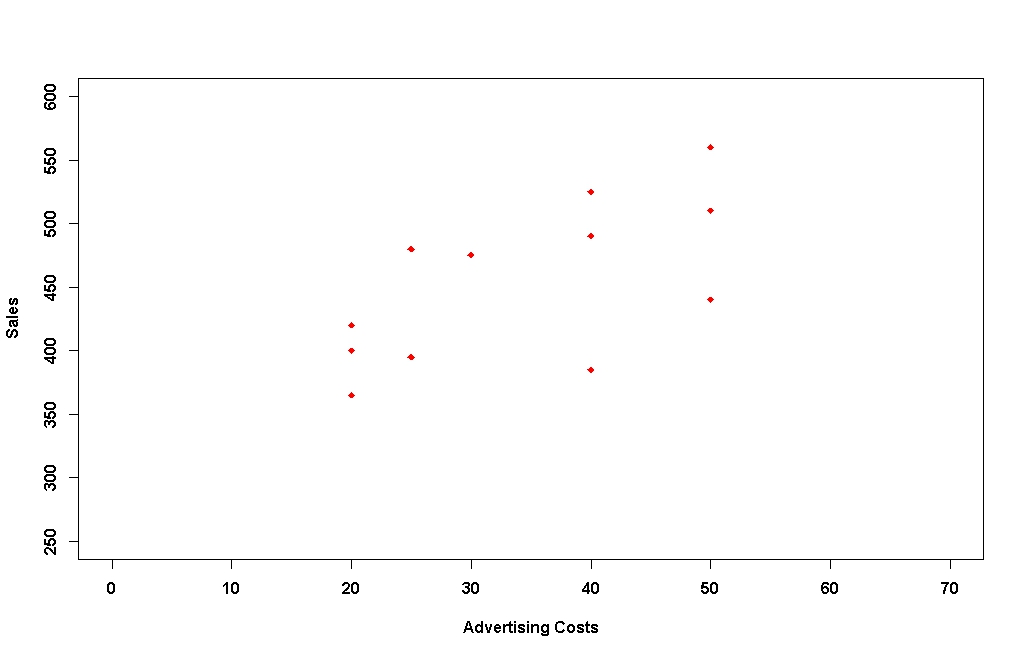
\includegraphics[scale=0.3]{images/12Bplot1.jpeg}\\
	\end{figure}
\end{center}

%%%%%%%%%%%%%%%%%%%%%%%%%%%%%%%%%%%%%%%%%%%%%%%%%%%%%%%%%%%%%%%%%%%%%%%%%


Summations
\begin{itemize}
	\item $\sum X$ = 410
	\item $\sum Y$ = 5445
	\item $\sum X^2$ = 15650
	\item $\sum Y^2$ = 2512925
	\item $\sum XY$ = 191325
\end{itemize}
Mean Values
\begin{itemize}
	\item $\bar{x}$ = 34.16
	\item $\bar{y}$ = 453.75
\end{itemize}


%%%%%%%%%%%%%%%%%%%%%%%%%%%%%%%%%%%%%%%%%%%%%%%%%%%%%%%%%%%%%%%%%%%%%%%%%

Sums of Squares Identities
\begin{itemize}
	\item $S_{XX}$ = 1641.67
	\item $S_{YY}$ = 42256.25
	\item $S_{XY}$ = 5287.5
\end{itemize}
Pearson's Correlation Estimate
\[ r_{XY} = \frac{S_{XY}}{\sqrt{S_{XX} \times S_{YY}}} = \frac{5287.5}{\sqrt{1641.67 \times 42256.25}} = 0.6348 \]

Weak to strong positive linear relationship.

%%%%%%%%%%%%%%%%%%%%%%%%%%%%%%%%%%%%%%%%%%%%%%%%%%%%%%%%%%%%%%%%%%%%%%%%%

Regression Coefficients
\begin{itemize}
	\item Slope Estimate $b_1$ = $S_{XY}$/$S_{XX}$ = 5287.5 / 1641.67 = 3.221
	\item Intercept Estimate $b_0$ = $\bar{y} - b_1 \times \bar{x}$ = $453.75-(3.221\times 34.16)$ = 343.70
\end{itemize}
Regression Equation
\[ \hat{y} = 343.70 + 3.221x \]


%%%%%%%%%%%%%%%%%%%%%%%%%%%%%%%%%%%%%%%%%%%%%%%%%%%%%%%%%%%%%%%%%%%%%%%%%

\begin{center}
	\begin{figure}
		% Requires \usepackage{graphicx}
		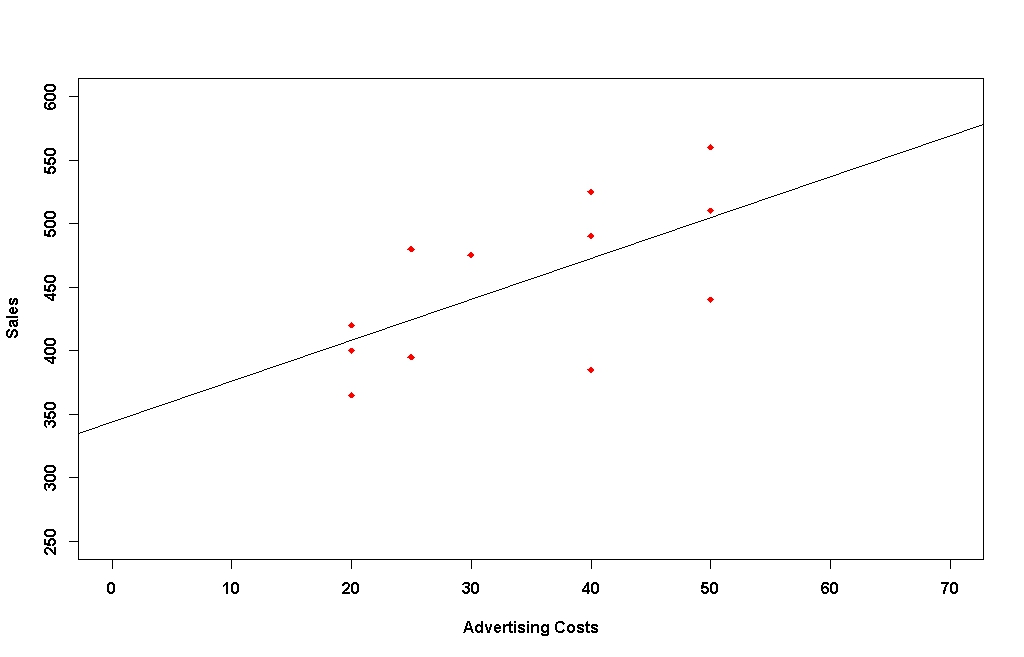
\includegraphics[scale=0.3]{images/12Bplot2.jpeg}\\
	\end{figure}
\end{center}

%%%%%%%%%%%%%%%%%%%%%%%%%%%%%%%%%%%%%%%%%%%%%%%%%%%%%%%%%%%%%%%%%%%%%%%%%


Estimate weekly sales when advertising costs are 35,000 (i.e X=35).
\[ \hat{y} = 343.70 + 3.221x \]

\[ \hat{y}_{X=35} = 343.70 + 3.221(35)  = 456.4 \]

When the advertising costs are 35,000, the expected sales are predicted to be 456,400.

Estimate weekly sales when advertising costs are 40,000 (ie. X=40).


\[ \hat{y}_{X=35} = 343.70 + 3.221(40)  = 472.54 \]

When the advertising costs are 40,000, the expected sales are predicted to be 472,540.


\subsubsection{Regression Example}

Predicted and Observed values
\begin{itemize}
	\item In simple linear regression, we predict scores on one variable from the scores on a second variable.
	\item In the last example, we predicted the value of sales to be 472.54 the costs were X=40.
	\item In fitting the model, we used three observations when the value of X was 40 (i.e. Y = 385,490,525)
	\item These are observed values, used to compute the model, and are distinct from predicted values $\hat{y}$.
	\item The predicted values are estimates for future observations
	\item The difference between an observed value and it's corresponding predicted value is known as a \textbf{\textit{residual}}.
	\[e_i = y_i-\hat{y}_i \]
	\item As there are three observations at X=40, there are three residuals.
\end{itemize}





\section*{Ansombe's Quartet}
\begin{tabular}{||c|c||c|c||c|c||c|c||}
	\hline
	Set 1 	&		&	Set 2	&		&	Set 3	&		&	Set 4	&		\\
	x	&	y	&	x	&	y	&	x	&	y	&	x	&	y	\\
	10	&	8.04	&	10	&	9.14	&	10	&	7.46	&	8	&	6.58	\\
	8	&	6.95	&	8	&	8.14	&	8	&	6.77	&	8	&	5.76	\\
	13	&	7.58	&	13	&	8.74	&	13	&	12.74	&	8	&	7.71	\\
	9	&	8.81	&	9	&	8.77	&	9	&	7.11	&	8	&	8.84	\\
	11	&	8.33	&	11	&	9.26	&	11	&	7.81	&	8	&	8.47	\\
	14	&	9.96	&	14	&	8.1	&	14	&	8.84	&	8	&	7.04	\\
	6	&	7.24	&	6	&	6.13	&	6	&	6.08	&	8	&	5.25	\\
	4	&	4.26	&	4	&	3.1	&	4	&	5.39	&	19	&	12.5	\\
	12	&	10.84	&	12	&	9.13	&	12	&	8.15	&	8	&	5.56	\\
	7	&	4.82	&	7	&	7.26	&	7	&	6.42	&	8	&	7.91	\\
	5	&	5.68	&	5	&	4.74	&	5	&	5.73	&	8	&	6.89	\\
	\hline
\end{tabular}






{Regression : Least Square Estimation}
It can be shown, using differential calculus that the values of $b_0$
and $b_1$ that best estimate the true parameters $\beta_0$ and $\beta_1$ are:

\[ b_1 = \frac{S_{XY}}{S_{XX}}\]
and
\[ b_0 = \bar{y} - b_1 \bar{x} \]

$\bar{x}$ and $\bar{x}$ are the sample means of X and Y respectively.


			\section*{May 2013 Question 6b Correlation and Regression }
			Calculate the correlation coefficient and interpret the value.
			\begin{tabular}{|c|c|c|}
				\hline Residence	& X	  & Y \\ 
				\hline  &  &  \\ 
				\hline  &  &  \\ 
				\hline 
			\end{tabular} 
			
			%-------------------------------------------------%
			
			\section*{Theory Components}
			\begin{itemize}
				\item Distinguish between a bimodal distribution and a unimodal distribution
				\item Compare and contrast interval and ordinal data.
			\end{itemize}







\subsubsection{Regression Example}
Scatterplot: Indicates a weak positive linear relationship.
\begin{center}
	\begin{figure}
		% Requires \usepackage{graphicx}
		\includegraphics[scale=0.3]{images/12Bplot3.jpeg}\\
	\end{figure}
\end{center}



\subsubsection{Regression Example}

Predicted and Observed Values

\begin{center}
	\begin{tabular}{|c|c|c|c|}
		\hline
		% after \\: \hline or \cline{col1-col2} \cline{col3-col4} ...
		X & Y& $\hat{y}$ & $e_i$ \\
		40 &385 &472.54 &-87.54\\
		40 &490 &472.54 & 17.46\\
		40 &525 &472.54 & 52.46\\
		\hline
	\end{tabular}
\end{center}


			
			\section*{May 2012 Question 2 Correlation and Regression}
			\begin{itemize}
				\item The sample size $n$ = 10.
				\item The \textbf{\textit{independent}} variable, usually denoted $x$, is the "cause variable" or "predictor variable".
				\item The \textbf{\textit{dependent}} variable, usually denoted $y$, is the "effect variable".
				\item Here the Maths achievement test score is the independent variable and the final grade in statistics is the dependent variable.
				\item A big hint is given in the notation of the question.
			\end{itemize}
			
			% X = c(39,43,21,64,57,47,28,75,34,52)
			% Y = c(65,78,52,82,92,89,73,98,56,75)

	
	
	\textbf{Regression Example}
	Estimate weekly sales when advertising costs are 35,000 (i.e X=35).
	\[ \hat{y} = 343.70 + 3.221x \]
	
	\[ \hat{y}_{(X=35)} = 343.70 + 3.221(35)  = 456.4 \]
	
	When the advertising costs are 35,000, the expected sales are predicted to be 456,400.
	
	Estimate weekly sales when advertising costs are 40,000 (ie. X=40).
	
	
	\[ \hat{y}_{(X=40)} = 343.70 + 3.221(40)  = 472.54 \]
	
	When the advertising costs are 40,000, the expected sales are predicted to be 472,540.
	
	
	\textbf{Regression Example}
	
	Predicted and Observed values
	\begin{itemize}
		\item In simple linear regression, we predict scores on one variable from the scores on a second variable.
		\item In the last example, we predicted the value of sales to be 472.54 the costs were X=40.
		\item In fitting the model, we used three observations when the value of X was 40 (i.e. Y = 385,490 and 525)
		\item These are observed values, used to compute the model, and are distinct from predicted values $\hat{y}$.
		\item The predicted values are estimates for future observations
		\item The difference between an observed value and it's corresponding predicted value is known as a \textbf{\textit{residual}}.
		\[e_i = y_i-\hat{y}_i \]
		\item As there are three observations at X=40, there are three residuals.
	\end{itemize}
	
	
%	%%%%%%%%%%%%%%%%%%%%%%%%%%%%%%%%%%%%%%%%%%%%%%%%%%%%%%%%%%%%%%%%%%%%%%%%%
%	
%	\textbf{Regression Example}
%	Scatterplot: Indicates a weak positive linear relationship.
%	\begin{center}
%		\begin{figure}
%			% Requires \usepackage{graphicx}
%			\includegraphics[scale=0.3]{12Bplot3.jpeg}\\
%		\end{figure}
%	\end{center}
%	
	
	

	
	\begin{center}
		\begin{tabular}{|c|c|c|c|}
			\hline
			% after \\: \hline or \cline{col1-col2} \cline{col3-col4} ...
			X & Y& $\hat{y}$ & $e_i$ \\
			40 &385 &472.54 &-87.54\\
			40 &490 &472.54 & 17.46\\
			40 &525 &472.54 & 52.46\\
			\hline
		\end{tabular}
	\end{center}
	
	
	
	\textbf{Important Assumptions of Least Squares Regression}
	It is assumed that
	\begin{itemize}
		\item The residuals are independent and normally distributed,
		\item The residuals are normally distributed with mean zero,
		\item The residuals is independent of X.
		\item The variance of residuals is consistent across the range of X (Heteroscedascity).
	\end{itemize}
	If these assumptions are not met, then Least Squares regression is not appropriate as a solution, and other alternatives must be used (Not Part of Course).
	
	%%%%%%%%%%%%%%%%%%%%%%%%%%%%%%%%%%%%%%%%%%%%%%%%%%%%%%%%%%%%%%%%%%%%%%%%%
	





%-------------------------------------------------%
% R Code
%
% X = c(10, 15, 20, 25, 30, 35, 40)
% Y = c(11, 19, 34, 52, 58, 81, 109)
% plot(X,Y,pch=18,col="red",font.lab=2,main="Scatter Plot of X and Y")
% cor(X,Y) =0.9830478



%---------------------------------------------------------- %
\subsection*{Sums of Squares Identities}
Before we do anything, We need to compute the following sums of squares identities
\begin{itemize}
	\item $s_{xx}$
	\item $s_{yy}$
	\item $s_{xy}$
\end{itemize}
\subsection*{Calculation 1}
\[ s_{xx}  = \sum(x^2) - \frac{\sum(x)^2}{n} \]
\[ s_{xx}  = 23.634 - \frac{\sum(x)^2}{10} \]

\subsection*{Calculation 2}
\[ s_{yy}  = \sum(y^2) - \frac{\sum(y)^2}{n} \]
%\[ s_{xx}  = 23.634 - \frac{\sum(x)^2}{10} \]


\subsection*{Calculation 3}
\[ s_{xy}  = \sum(xy) - \frac{\sum(x)\times \sum{y}}{n} \]
%\[ s_{xx}  = 23.634 - \frac{\sum(x)^2}{10} \]

%------------------------------------------------------------%

\subsection*{Part iv - Prediction}
\begin{itemize}
	\item Suppose the regression equation is as follows
	\[ \hat{y} = 40.78424 + 0.76556 x \]
	\item If a student scored 5 marks on the achievement test (i.e. $x=5$), predict the students statistics grade.
	
	\[ \hat{y}_{(x=5)} = 40.78424 + (0.76556 \times 5) \]
	
	\item Solving using a calculator we get
	\[ \hat{y}_{(x=5)} = 44.61204 \]
	
	\item The score should be approximately 44.61.
\end{itemize}




\section{Regression}

The argument to lm is a model formula in which the tilde symbol
(~) should be read as ``described by”.


This was seen several times earlier, both in connection with
boxplots and stripcharts and with the t and Wilcoxon tests.



\section{Multiple Linear Regression}
The \texttt{lm()} function handles much more
complicated models than simple linear regression. There can be many other things besides a dependent and a descriptive variable in a model formula.

A multiple linear regression analysis (which we discuss in Chapter
11) of, for example, y on x1, x2, and x3 is specified as $y ~ x1 +
x2 + x3$.


This is an F test for the hypothesis that the regression coefficient is zero. This test is not really interesting in a
simple linear regression analysis since it just duplicates information already given—it becomes more interesting when there is more than one explanatory variable.







\section*{Linear Regression}
\begin{itemize}
	\item Linear regression is the most widely used of all statistical techniques: it is the study of linear (i.e., straight-line) relationships between variables, usually under an assumption of normally distributed errors.
\end{itemize}

\subsection{Regression}

\begin{verbatim}
> lm(short.velocity~blood.glucose)
\end{verbatim}





\textbf{Least Squares}
The method of least squares is a criterion for fitting a specified model to observed data.
For example, it is the most commonly used method of defining a straight line through a set of points on a scatterplot.





%---------------------------------------------------------------------%




The line is called the sample regression line of y on x.

The following example demonstrates the calculation of a and b and the use of the resultant
equation to estimate y for a given x.






%------------------------------------------------------------------------------------------------%
\subsection{R square}
The model with the highest R2 and adjusted R2  is the preferable of all candidate models
The quadratic model is the preferable model in that case.





					\end{document} 
